\subsection{IMU Testing}
The PmodNAV IMU is a small device that can be directly connected to the ZedBoard's Pmod connector. As such, it requires no external power source or other intermediate connections.

\subsubsection{Communication Testing}
With the rangefinder connected to the ZedBoard's PS MIO Pmod, JE, the PmodNAV IMU requires an Extended MIO Pmod so that it could still be controlled by the PS. As such, the IMU's SPI pins were routed to the JD Pmod. Since the main point of communication with the IMU is its magnetometer, the IMU's slave select and register settings were adjusted accordingly, as discussed in Section \ref{imu_settings}. To choose the magnetometer and deselect the accelerometer/gyroscope and barometer, the magnetometer's slave select was brought low for each SPI transfer while the other two were left high. The behavior of Pmod JD's pins were observed with an oscilloscope during an SPI transfer. We noticed that as soon as the magnetometer's slave select line was asserted there was unidentified behavior with all of the other pins. Since the IMU was disconnected we believed this issue to be with routing the SPI pins to EMIO incorrectly, so we decided to test the SPI transfer via Pmod JE.
\par
The pins were re-routed to the MIO Pmod JE and more undefined functionality was observed when the magnetometer's slave select line was asserted. The ZedBoard's SPI errata was investigated until we found AR\# 47511, which describes an unresolved issue in the MIO interface where the SPI controller resets itself when slave select 0 signals asserts \cite{zedboardErrata}. This errata was the cause of the EMIO's undefined behavior too, since this issue affects the SPI controller itself.
\par
Luckily, the PmodNAV supports I\textsuperscript{2}C communication, too. To avoid this errata entirely I\textsuperscript{2}C was used and routed to Pmod JD. We began testing the IMU's I\textsuperscript{2}C behavior only to realize that the PmodNAV's magnetometer is inaccessible through the I\textsuperscript{2}C bus, which is undocumented in the device's datasheet \cite{lsm9ds1}. As such, SPI needs to be implemented.
\par
The SPI pins were again routed to Pmod JD. Attempting to avoid the errata, slave select 1 was assigned to the magnetometer. The other two slave select pins were routed away from Pmod JD so that they would not be configured or used in any manner. In their place are two GPIO pins configured as pull-ups so that these pins would idle high and never had to be written to. This setup was configured in Vivado's Synthesis tab, as shown in Figure \ref{emio_config}. 

\begin{figure}[H]
	\centerline{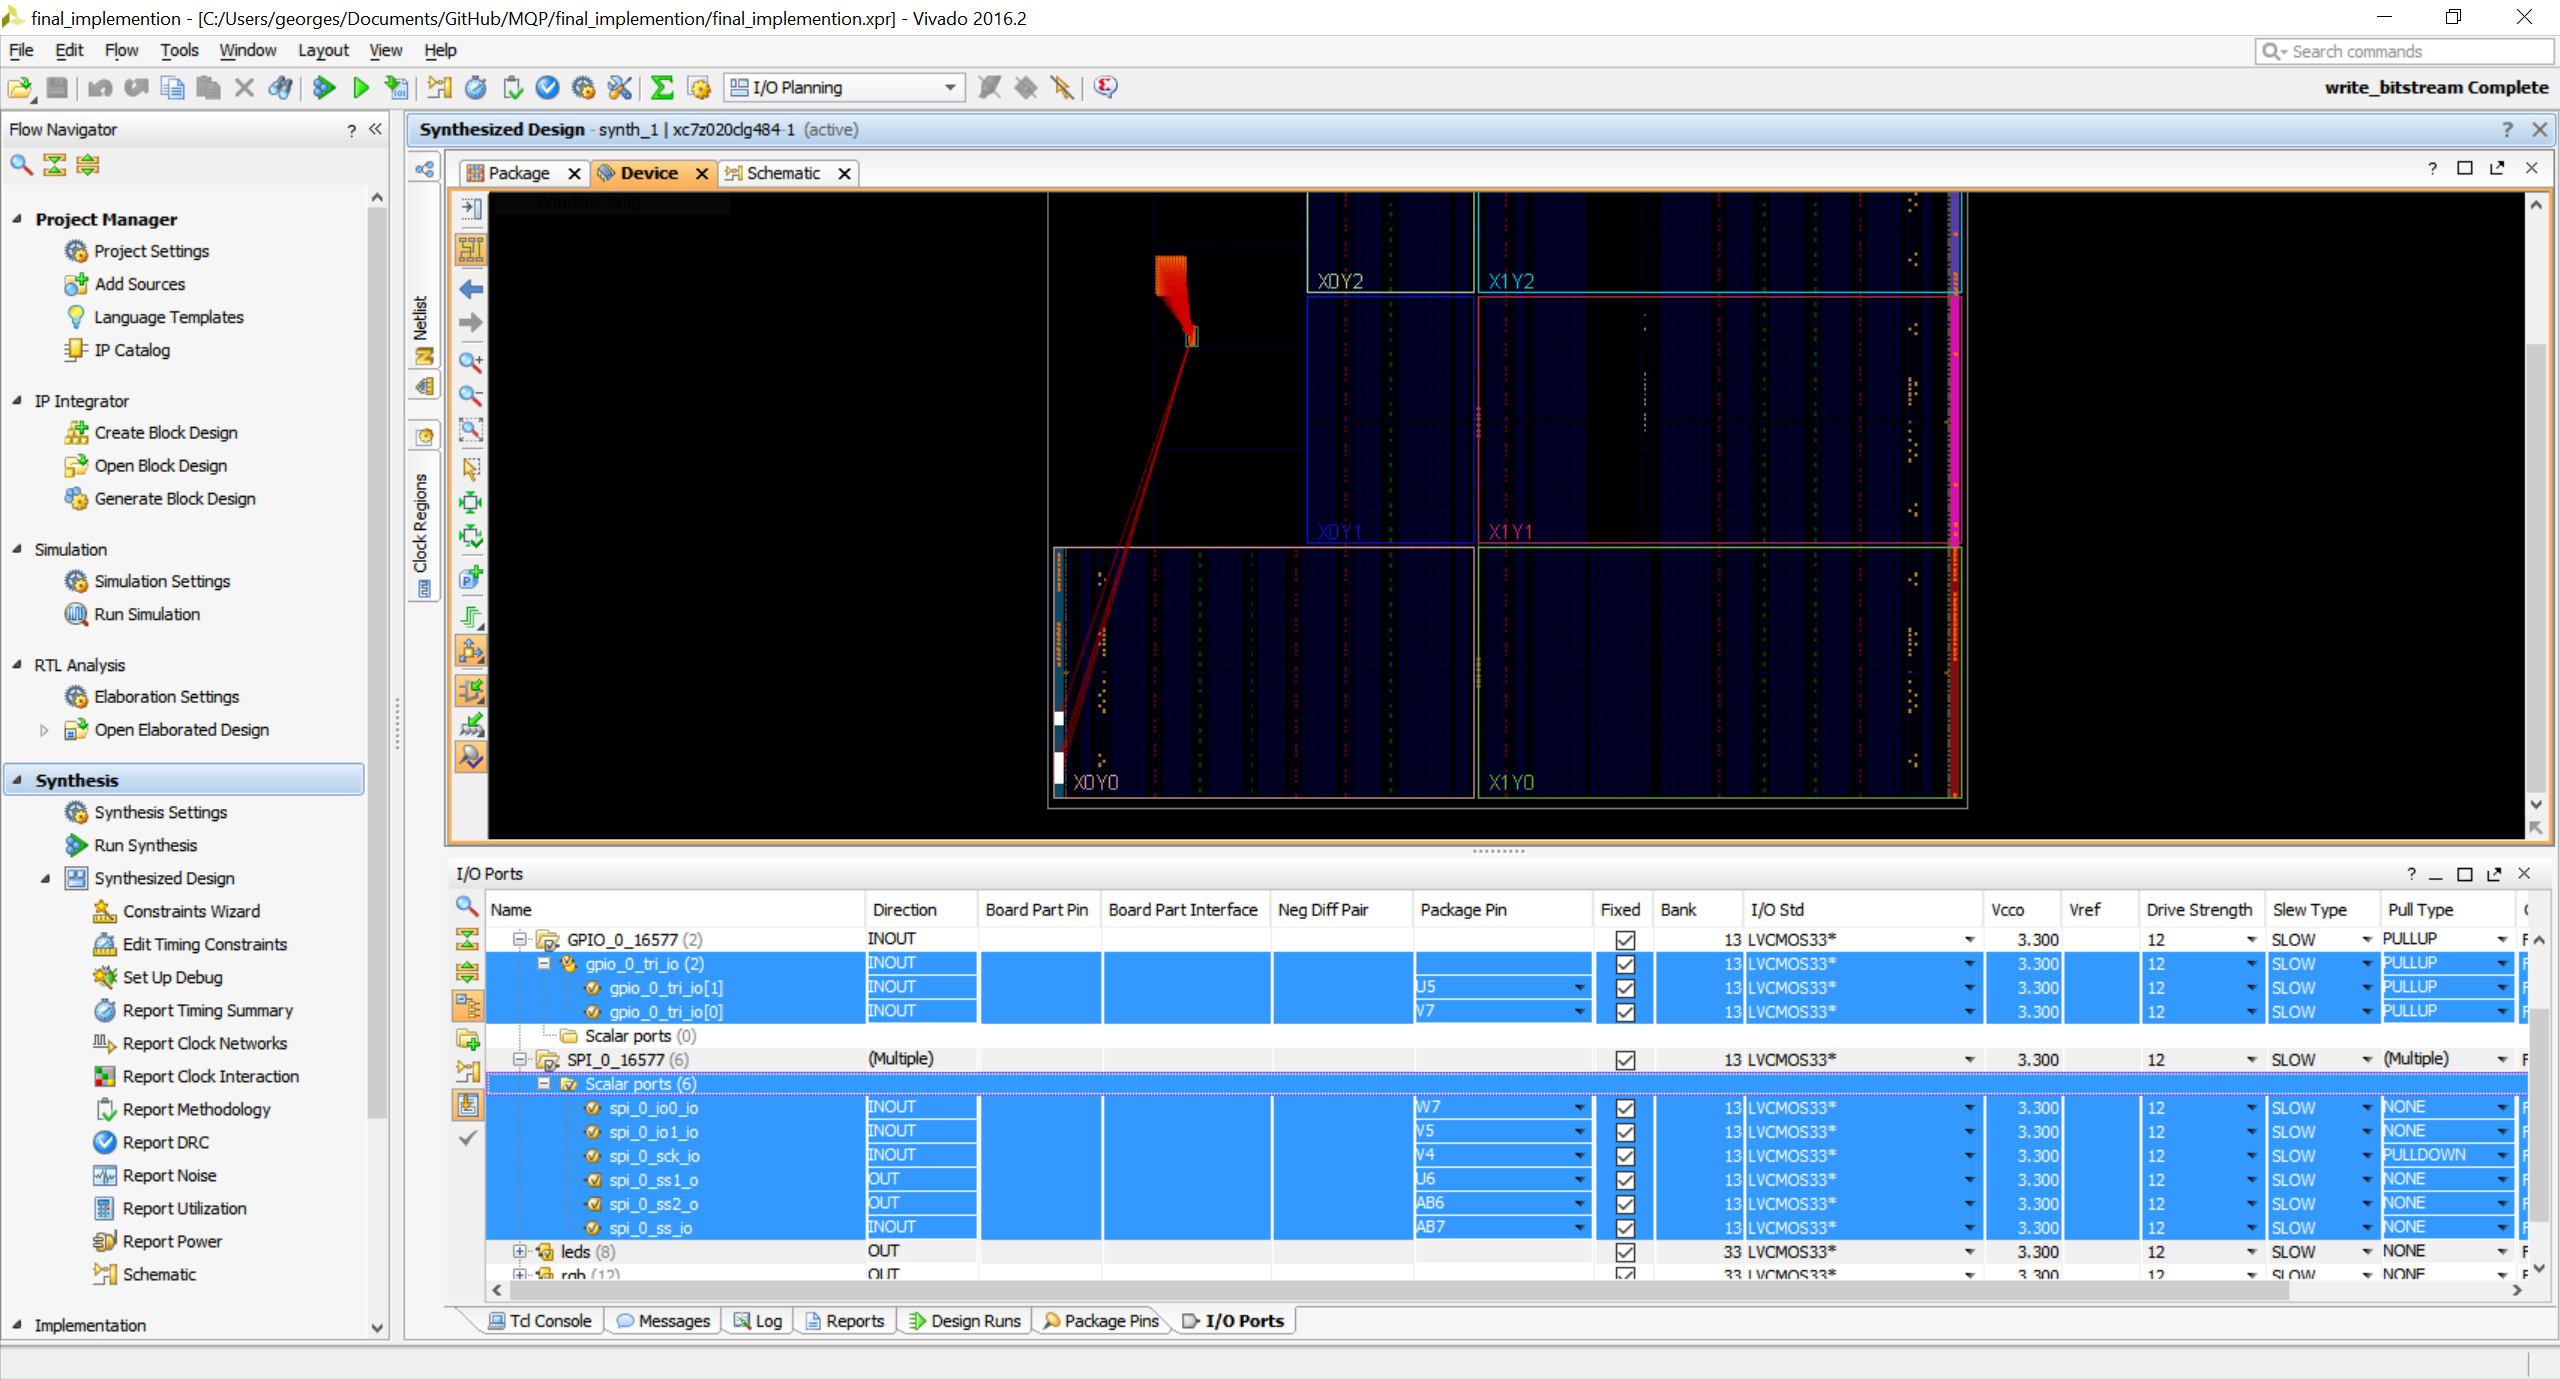
\includegraphics[width=1.1\textwidth]{editing_emio_pins.png}}
	\caption{EMIO SPI Configuration for PmodNAV}
	\label{emio_config}
\end{figure}

With this configuration a waveform similar to the correct waveforms, shown in Figures \ref{magnetometer_spi} and \ref{multiple_reads}, were observed. The IMU was connected to the ZedBoard and successful communication was observed on the oscilloscope, as shown in Figure \ref{OTPHJ}.

\begin{figure}[H] 
	\begin{subfigure}{1\textwidth}
	\centering
		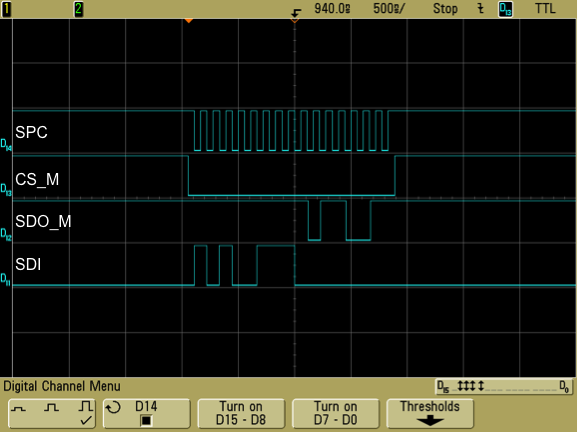
\includegraphics[width=0.75\linewidth]{magSingleRead_label.png}
		\caption{IMU Magnetometer Single Read Operation}
	\end{subfigure}
	\begin{subfigure}{1\textwidth}
	\centering
		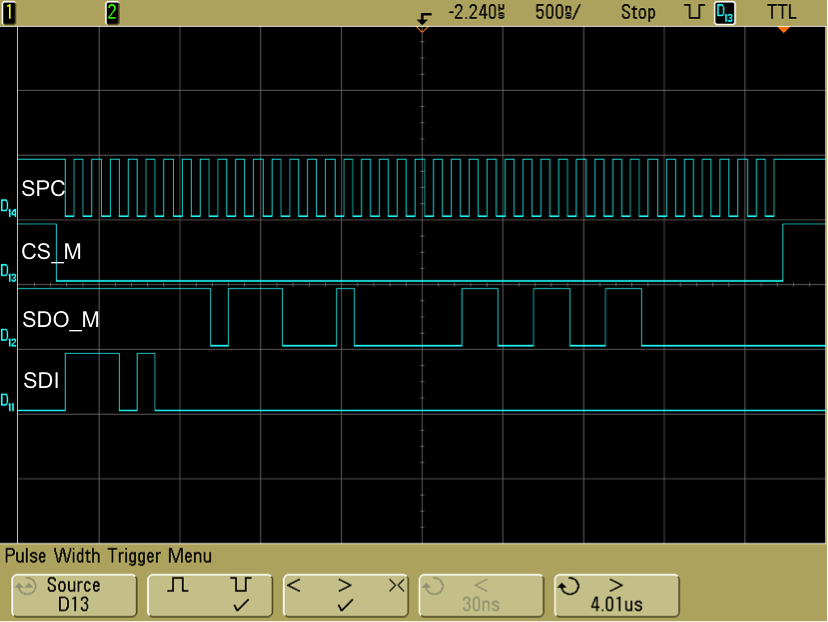
\includegraphics[width=0.75\linewidth]{magMultRead_label.png}
		\caption{IMU Magnetometer Multiple-Byte Read Operation}
	\end{subfigure}
	\caption{Successful IMU Communication via EMIO SPI}
	\label{OTPHJ}
\end{figure}

\subsubsection{Data Testing}
The IMU's data was tested by transmitting it via UART. The IMU's magnetometer data was processed until it was transformed into a compass heading. The ZedBoard's UART was routed to USB UART so that it could connect with a serial console. The ZedBoard, with the IMU connected, was rotated while the compass heading was being observed. The results were inaccurate and inconsistent until the ZedBoard was moved as far from the lab bench as the wires would allow. An IMU is a very sensitive piece of equipment that picks up electromagnetic interference, in this case most noticeably by the ZedBoard's own power supply. Once the device was further away from the lab bench, accurate and repeatable compass headings were observed. The further the ZedBoard and connected IMU are from the device's power supply, the better it performs.

\subsubsection{Interfacing with the ADIS16375 IMU}
Although we were ultimately able to interface with the PmodNAV IMU, this was not our first choice IMU. We originally attempted to interface with the ADIS16375 Six Degrees of Freedom Inertial Sensor, shown in Figure \ref{adis16375}.

\begin{figure}[H]
	\centerline{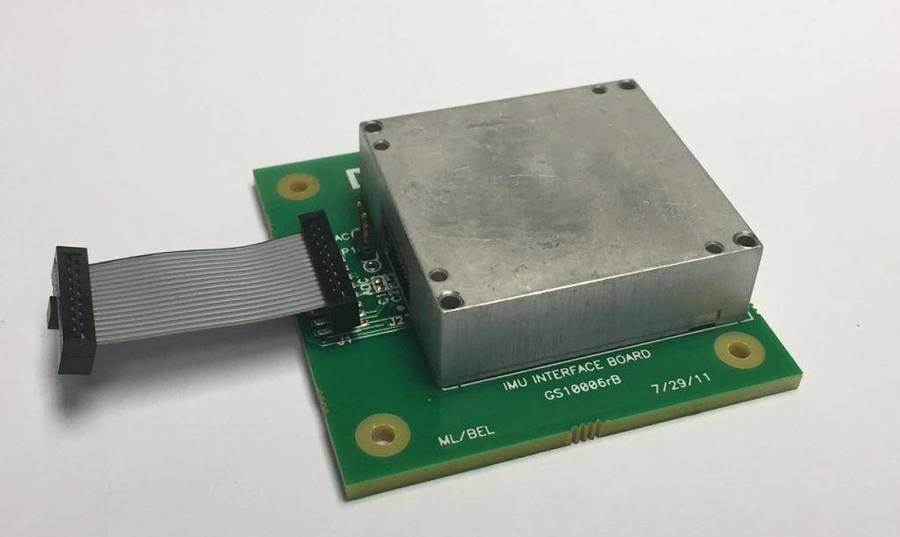
\includegraphics[width=.7\textwidth]{adis16375.jpg}}
	\caption{The ADIS16375 Six Degrees of Freedom Inertial Sensor \cite{adisBreakout}}
	\label{adis16375}
\end{figure}

This IMU is a highly sensitive, heavy duty device. It has a tri-axis gyroscope, a tri-axis accelerometer, and a temperature sensor, has onboard functionality to calculate delta-angle and velocity, and uses SPI communication. Although the ADIS16375 does not have a magnetometer, its gyroscope's sensitivity combined with its sample rate and onboard delta-angle calculation make it perfect to accommodate for device rotation. In addition, the device's onboard velocity calculation is extremely useful for displacement calculations. However, we were not able to communicate with it. There was no way to test the ADIS16375 so we could not verify it was functioning in any manner. With a strict deadline approaching, the PmodNAV was implemented as a quick and simple solution.




